\documentclass[aps,prc,reprint,amsmath,nofootinbib]{revtex4-1}

\usepackage{hyperref}
\usepackage{graphicx}
\usepackage{subcaption}
\usepackage{tabularx}
\graphicspath{{fig/}}

%\usepackage{tikz}
%\usetikzlibrary{shapes,calc,matrix}

%\usepackage{mdwlist}
%\renewcommand\labelitemi{\raisebox{.3ex}{\tiny$\bullet$}}

%\newcommand{\trento}{T\raisebox{-.5ex}{R}ENTo}
%\newcommand{\nch}{N_\text{ch}}
%\newcommand{\eccratio}{\sqrt{\langle \varepsilon_2^2 \rangle}/\sqrt{\langle \varepsilon_3^2 \rangle}^{\,0.6}}

\begin{document}

\title{Entropy deposition in ultra-relativisitic nucleus-nucleus collisions}

\author{J.\ Scott Moreland}
\date{\today}

\maketitle

\section{Introduction}

Microseconds after the big bang, our universe was super heated to several trillion kelvin. In these extreme conditions, nuclear matter melted to form a hot 
soup of subatomic quarks and gluons known as a quark-gluon plasma (QGP). As the universe expanded and cooled, these colored degrees of freedom recombined to 
form coloreless hadronic states (e.g. protons and neutrons) kickstarting the elaborate process of nucleosysnthesis.

Empirical evidence for this plasmonic state of nuclear matter was first provided by researchers at the Relativisitic Heavy-Ion Collider (RHIC) in Brookhaven, NY.
Collisions of ultra-relativistic gold nuclei at RHIC produced fireballs which exhibited strong signs of collective flow. These results were in stark contrast 
to low energy nuclear collisions at SPS which indicated only weak signs of collective behaviour and led RHIC scientists to announce indirect evidence for a new state
of matter.



\begin{figure*}[t]
  \centering
  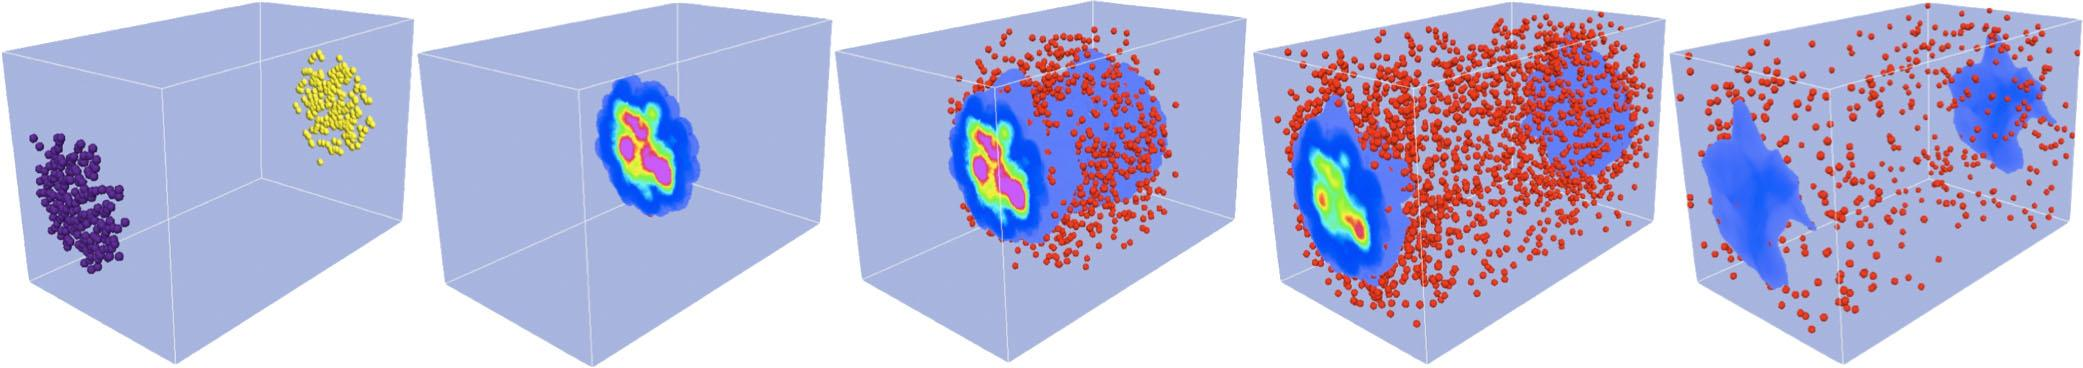
\includegraphics[width=\textwidth]{evolution} \\
  0 fm/c   \hspace{.13\textwidth}
  0.5 fm/c \hspace{.13\textwidth}
  8 fm/c   \hspace{.13\textwidth}
  16 fm/c  \hspace{.13\textwidth}
  22 fm/c
  \caption{Figure from \cite{iss}}
  \label{fig:coll}
\end{figure*}

\section{Relativisitic nuclear collisions}

\begin{figure*}
 \includegraphics[height=0.2\textwidth]{collision1}
 \includegraphics[height=0.2\textwidth]{collision2}
 \includegraphics[height=0.2\textwidth]{collision3}
 \includegraphics[height=0.2\textwidth]{collision4}
\end{figure*}

\section{Fluid dynamic simulations}

\begin{figure}
 \includegraphics[width=0.15\columnwidth]{e2-crop} \hspace{.01\columnwidth} 
 \includegraphics[width=0.23\columnwidth]{e3-crop} \hspace{.01\columnwidth}
 \includegraphics[width=0.21\columnwidth]{e4-crop} \hspace{.01\columnwidth}
 \includegraphics[width=0.24\columnwidth]{e5-crop}\\
 \flushleft
 \vspace{-0.1in}
 \hspace{0.08\columnwidth} 2 \hspace{0.19\columnwidth} 3 \hspace{0.21\columnwidth} 4 \hspace{0.22\columnwidth} 5
 \caption{Diagrams of the second, third, fourth and fifth azimuthal Fourier harmonics. The angular resolution increases with increasing harmonic number.}
\end{figure}

\begin{figure*}
 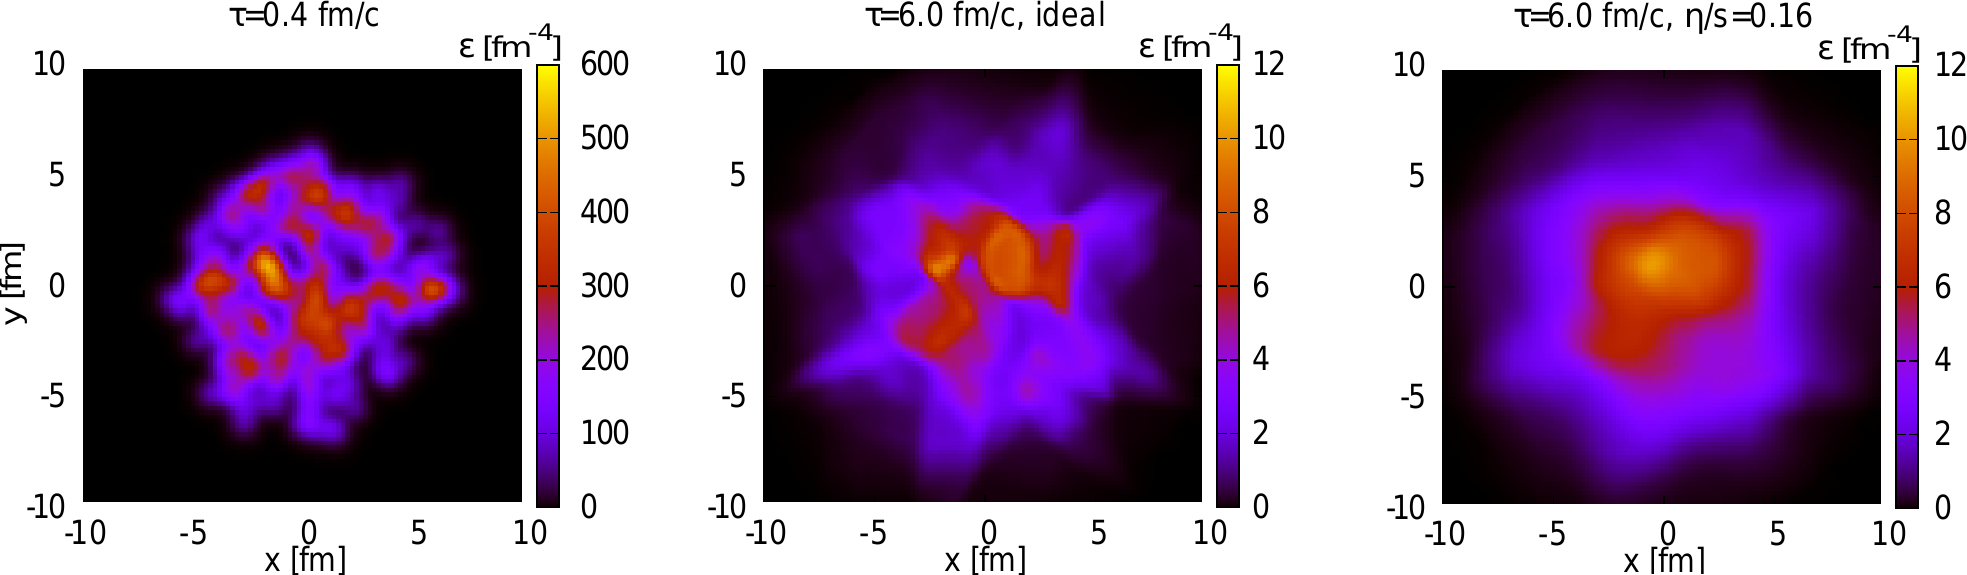
\includegraphics[width=\textwidth]{three}
\end{figure*}

\begin{figure}
 \includegraphics[height=0.19\textwidth]{motivation1-crop}\\
 \includegraphics[height=0.13\textwidth]{motivation2-crop}
\end{figure}

\begin{figure}
 \includegraphics[width=\columnwidth]{saturation}
\end{figure}

\begin{figure}
 \includegraphics[width=\columnwidth]{trento-profiles}
\end{figure}


\begin{figure*}
 \includegraphics[width=\textwidth]{multdist}
\end{figure*}

\begin{figure*}
 \includegraphics[width=\textwidth]{eccentricity}
\end{figure*}

\bibliography{prelim,duke-qcd-refs/Duke_QCD_refs}


\end{document}
